\documentclass{article}
\usepackage[utf8]{inputenc}
\usepackage[slovene]{babel}
\usepackage{graphicx}
\usepackage{subfigure}
\usepackage{amsfonts} 
\usepackage{amsmath}
\usepackage{hyperref}

\newcommand{\program}{Finanča matematika} 
\newcommand{\imeavtorja}{Anja Plesec}
\newcommand{\imementorja}{prof.~dr.~ Sergio Cabello Justo, \\ asist. Gašper Domen Romih}
\newcommand{\naslovdela}{Gradientni spust}
\newcommand{\letnica}{2022}

\begin{document}

\thispagestyle{empty}
\noindent{\large
UNIVERZA V LJUBLJANI\\[1mm]
FAKULTETA ZA MATEMATIKO IN FIZIKO\\[5mm]
\program\ -- 2.~stopnja}
\vfill

\begin{center}{\large
\imeavtorja\\[2mm]
{\bf \naslovdela}\\[10mm]
Končno poročilo pri predmetu Matematika z računalnikom\\[1cm]
Mentor: \imementorja}
\end{center}
\vfill

\noindent{\large
Ljubljana, \letnica}
\pagebreak

\newpage



\section{Gradientni spust}
Gradientni spust je iterativna metoda za iskanje lokalnega minimuma funkcije. To je algoritem, ki se lahko uporablja na različnih področjih. Cilj pa je imeti algoritem s čim manj iteracij. \\

Samo delovanje algoritma je sledeče. Najprej si izberemo začetno točko (initial value) - $x_0 \in \mathbb{R}^n $ in hitrost konvergence (learning rate). Zapišemo stroškovno funkcijo (Loss Function) in jo odvajamo po vseh parametrih. Na ta način dobimo gradient stroškovne funkcije. Izbrano začetku točko nato vstavimo v ta gradient in s pomočjo tega poračunamo velikost naslednjega koraka:
$$ \text{velikost koraka} = \nabla f(x_t) \cdot \text{learning rate} $$
Vrednost novega parametra pa dobimo s pomočjo spodnje formule:
$$ x_1 = x_0 - \text{velikost koraka} \in \mathbb{R}^n$$
Ko izračunamo vrednost $x_1$ postopek ponovimo.\\

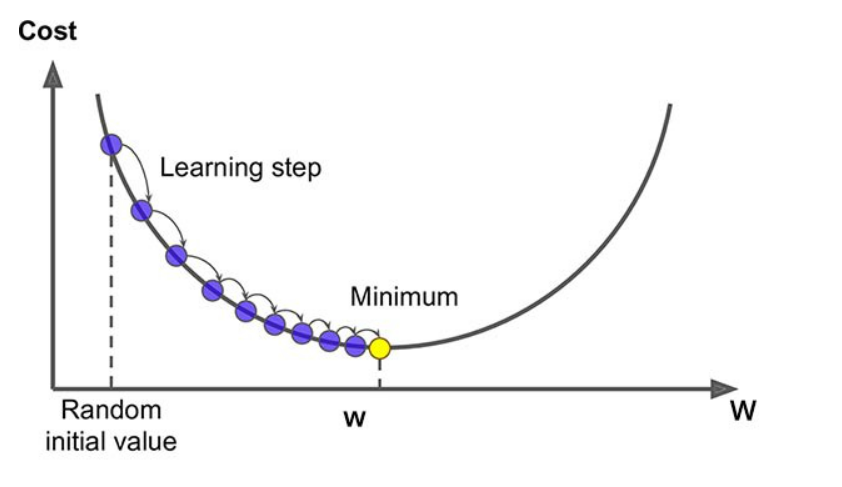
\includegraphics[scale=0.6]{grad_des}
\newline

Splošen algoritem:
\begin{itemize}
\item{Izberemo začetno točko $x_0 \in \mathbb{R}^n $. }
\item{Za $t \geq 0$ predpostavimo, da poznamo $x_0,x_1, \ldots ,x_t $. Naslednji člen določimo s pomočjo enačbe: 
\[ x_{t+1}=x_t - \eta \cdot \nabla f(x_t), \] 
kjer $ \eta$ predstavlja learning rate, $\nabla f(x_t) $ pa gradient funkcije $f$ v točki $x_t$.}
\item{Končamo in vrnemo zadnjo iteracijo.}
\end{itemize}

Težave, ki se pri tem algoritmu pojavijo, so ustrezna izbira vhodnih podatkov. Eden izmed teh je ``learning rate''. Radi bi delali velike korake, kar bi pomenilo manjše število iteracij, vendar se nam lahko zgodi, da s tem zgrešimo našo rešitev in sam algoritem ne vrne prave rešitve. Naslednji izmed vhodnih podatkov je začetna točka $x_0$. Želimo si jo izbrati tako, da je čim bližje optimalni rešitvi, saj bomo zaradi tega potrebovali manj iteracij.\\

Projekt bom izdelala v programu Matlab.


\section{Primer uporabe pri linearni regresiji}
Gradientni spust doseže optimalno vrednost tako, da na začetku algoritma dela velike korake, ko pa se bliža optimalni vrednosti (minimumu) pa so koraki vedno manjši. To lastnost algoritma lahko potrdita tudi slika 1 in 2. Na prvi sliki torej vidimo, da pet dodatnih iteracij zelo vpliva na premico (razlika med pet in deset iteracij), med tem ko na drugi sliki, kjer gledamo razliko med 95 in 100 iteracij, skoraj ni razlike, saj so koraki, ki jih delamo vedno manjši. \\



\begin{figure}[h]
    \centering
    \subfigure{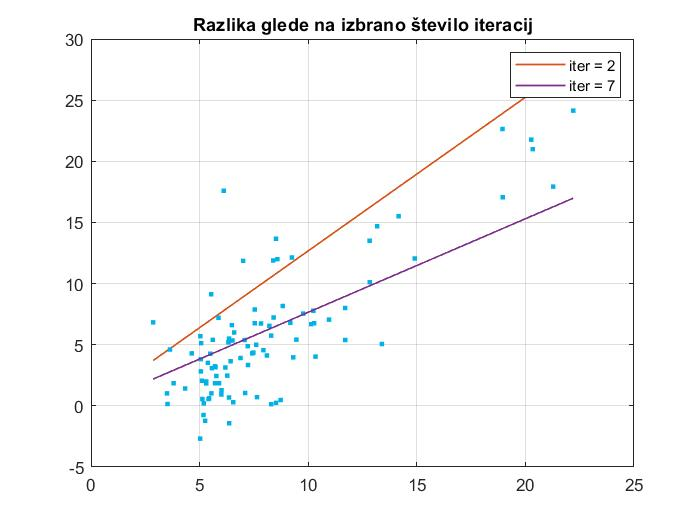
\includegraphics[width=0.45\textwidth]{premica_iter1.jpg}}
    \subfigure{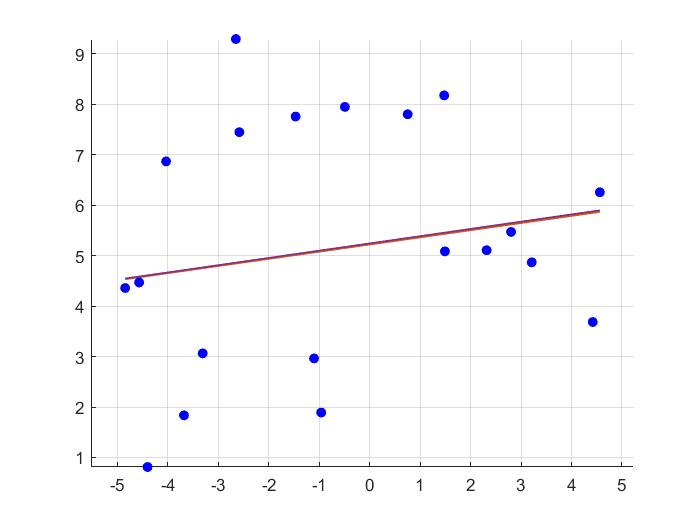
\includegraphics[width=0.45\textwidth]{premica_iter2.jpg}} 
    \caption{Razlike v velikosti koraka}
    \label{fig:foobar}
\end{figure}


\noindent Izvedla sem poskus, kjer sem spreminjala začetne pogoje in opazovala koliko iteracij je potrebno, da se premica približa optimalni rešitvi. V primeru a) sem vzela za parametra naklon in konstanta kar vrednost 1. Ko izvedemo 90 iteracij se zadnja iteracija dobro približa začetni rešitvi. Pri primeru b) sem vzela naklon = -20 in konst = 50. Opazimo, da je v tem primeru potrebnih 200 iteracij. Prav toliko jih je potrebnih v c) primeru, kjer sem vzela naklon = -200 in konst = 500. 

\begin{figure}
    \centering
    \subfigure[naklon = 1, konst = 1]{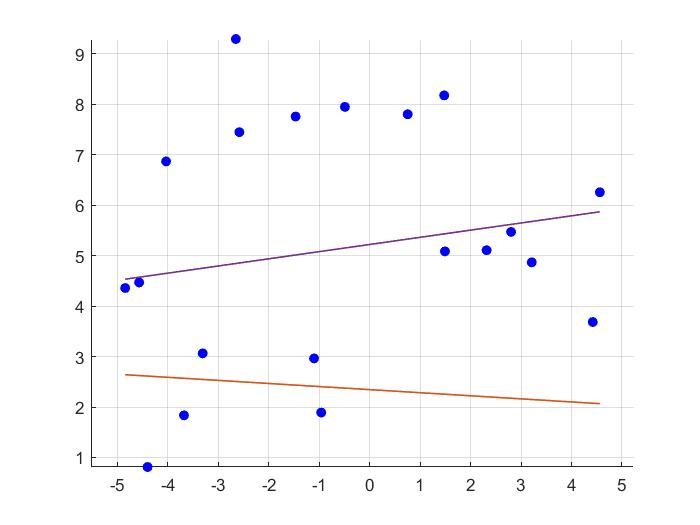
\includegraphics[width=0.45\textwidth]{premica_zp2.jpg}} 
    \subfigure[naklon = -20, konst = 50]{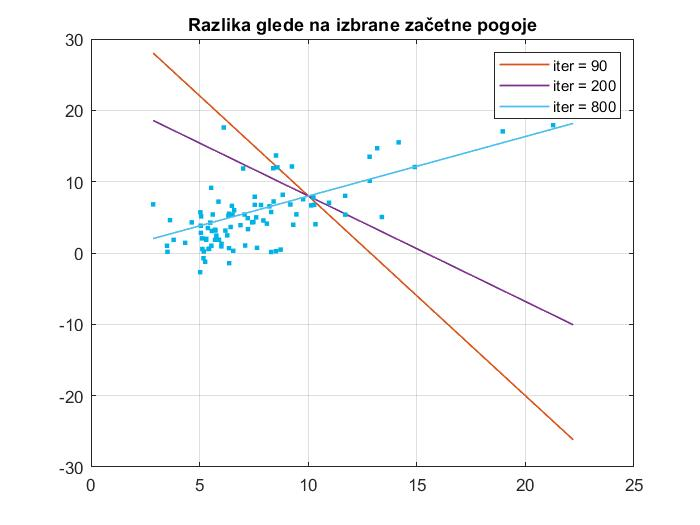
\includegraphics[width=0.45\textwidth]{premica_zp1.jpg}} 
    \subfigure[naklon = -200, konst = 500]{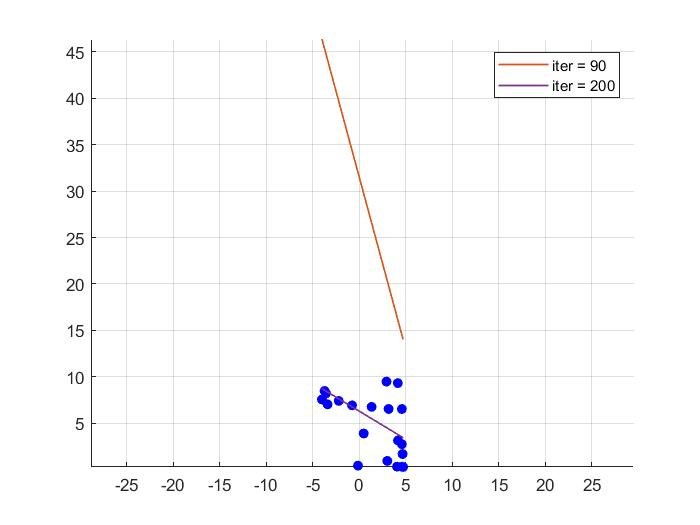
\includegraphics[width=0.45\textwidth]{premica_zp3.jpg}}
    \caption{Konvergenca pri različnih začetnih pogojih}
    \label{fig:foobar}
\end{figure}


\section{Iskanje minimuma podane funkcije}
\subsection{Iskanje minimuma funkcije ene spremenljivke}

Iz spodnjih slik lahko opazimo, da če izberemo preveliko učno stopnjo nam približki skačejo iz ene strani minimuma na drugo stran, med tem ko če izberemo manjšo nam približki ne skačejo. Opazimo, da pri preveliki in premajhni učni stopnji algoritem potrebuje več iteracij. Torej moremo izbrati ravno pravšnjo za našo metodo. Za začetni približek vzamemo $x_0 = 4$

\begin{figure}[h]
    \centering
    \subfigure{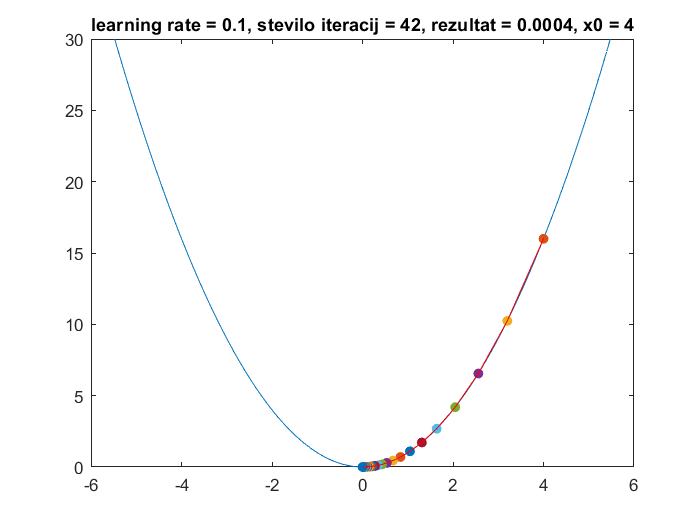
\includegraphics[width=0.45\textwidth]{fun_lepo.png}}
    \subfigure{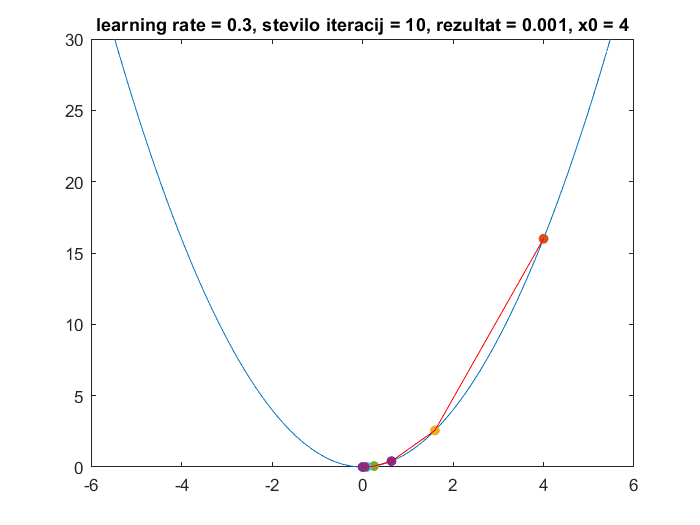
\includegraphics[width=0.45\textwidth]{fun_lepo2.png}} 
    \subfigure{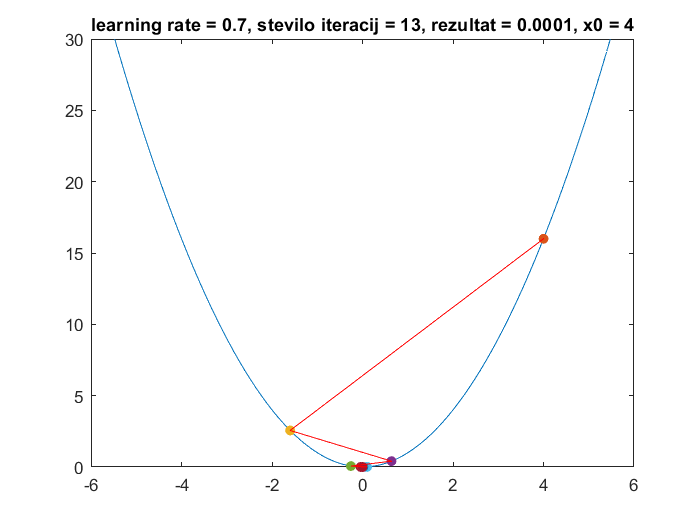
\includegraphics[width=0.45\textwidth]{fun_skace.png}}
    \subfigure{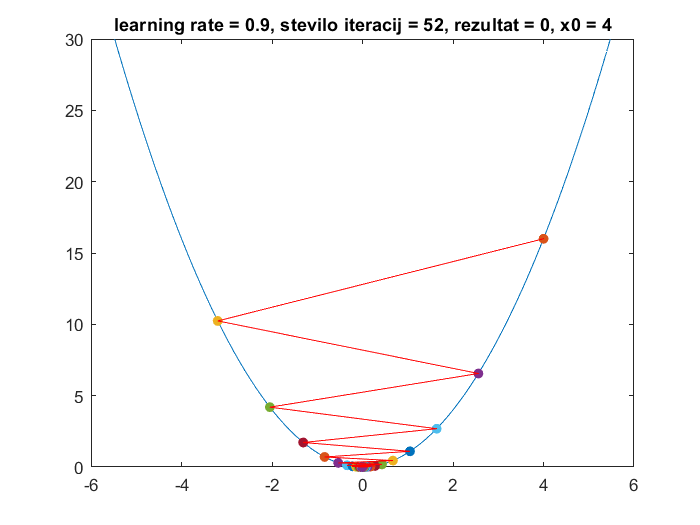
\includegraphics[width=0.45\textwidth]{fun_skace2.png}} 
    \caption{Razlike glede na izbrano učno stopnjo}
    \label{fig:foobar}
\end{figure}


\noindent Sam algoritem ni primeren za funkcije, ki je nekaj časa skoraj konstantna oz je naklon tangente skoraj ničelni. Pri takih funkcijah sam algoritem potrebuje veliko več iteracij, da pride do minimuma. Na spodnjem grafu funkcije $\frac{x^2}{1000}$ vidimo, da je kljub dobro izbrani učni stopnji končna vrednost približka za minimum 0.8066, ker je še vedno daleč stan od samega minimuma naredili pa smo 1000 iteracij.


\begin{figure}[h]
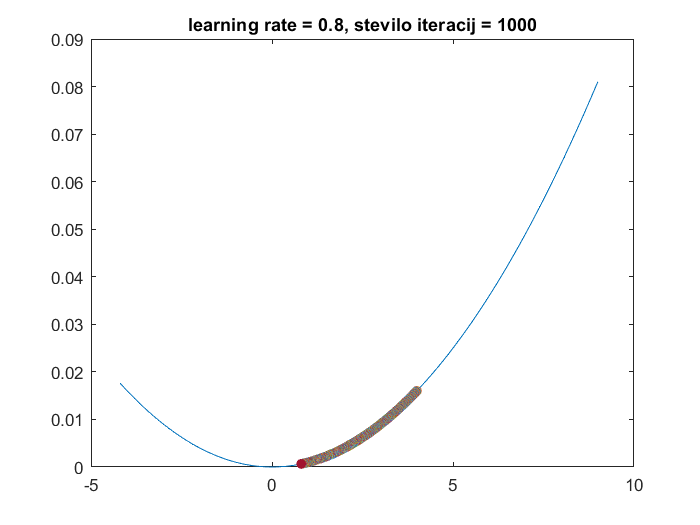
\includegraphics[scale=0.6]{izravnana_fun}   
 \caption{Izravnana funkcija}
\label{fig:foobar}
\end{figure}

\newpage
\noindent Zanimiv primer je naslednja funkcija $x^4-2x^3+2$. Težave algoritmu povzroči sedlo. Lahko vidimo kako izbira začetne točke in učne stopnje vplivata na rešitev algoritma. Seveda v primerih sedelne točke ne moremo trditi, da nam algoritem res vrne globalni minimum.\\
\begin{figure}[!htb]
    \centering
    \subfigure{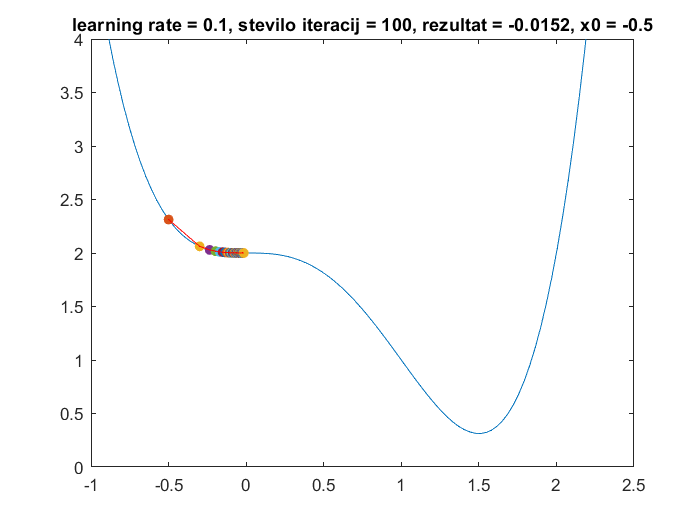
\includegraphics[width=0.45\textwidth]{sedlo1.png}}
    \subfigure{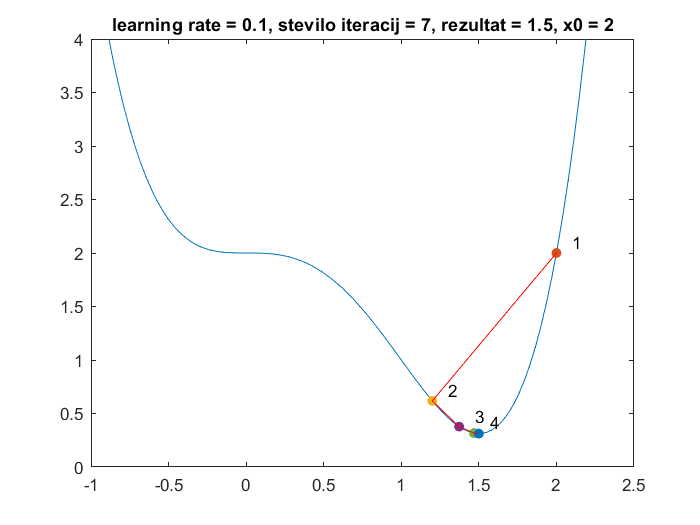
\includegraphics[width=0.45\textwidth]{sedlo2.png}} 
    \subfigure{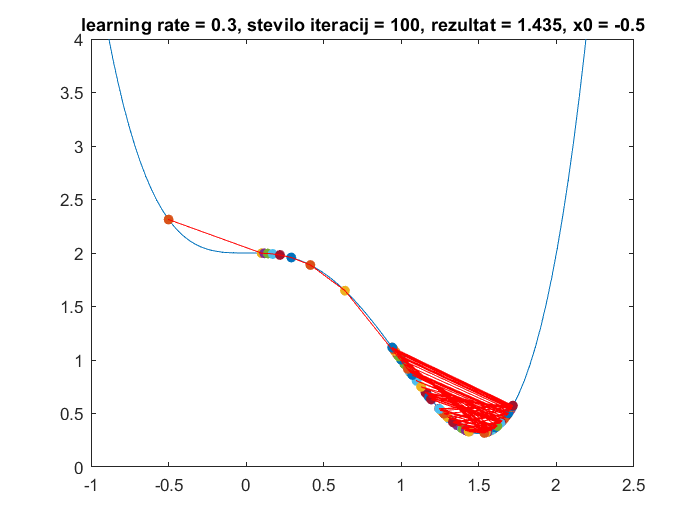
\includegraphics[width=0.45\textwidth]{sedlo3.png}}
    \subfigure{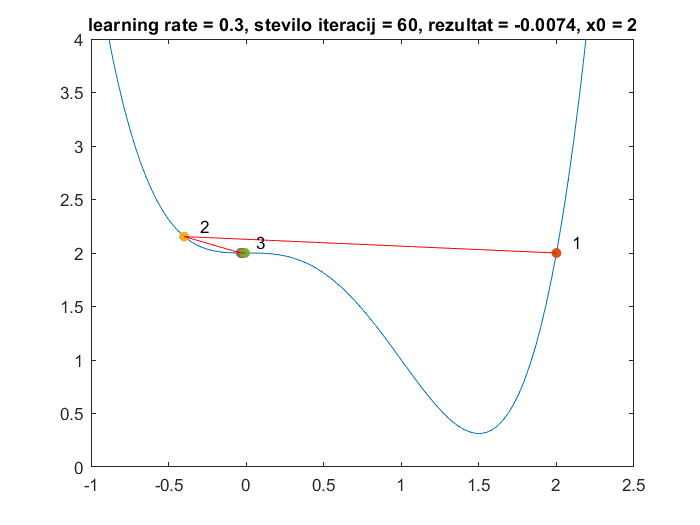
\includegraphics[width=0.45\textwidth]{sedlo4.png}} 
    \subfigure{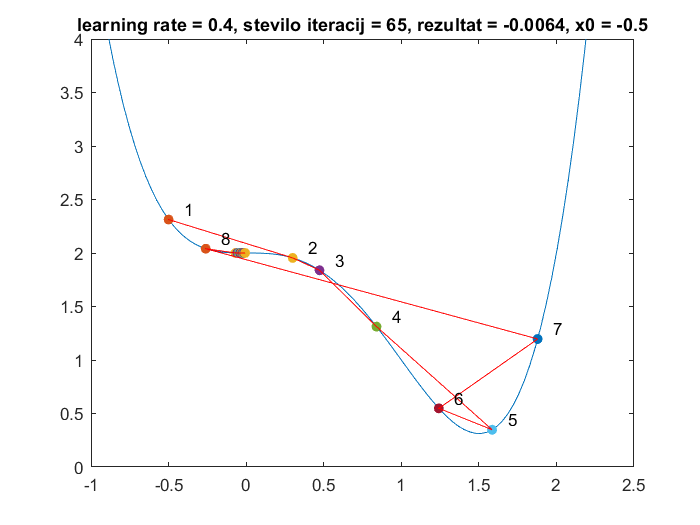
\includegraphics[width=0.45\textwidth]{sedlo5.png}} 
    \caption{Razlike glede na izbrano učno stopnjo in začetni približek}
    \label{fig:foobar}
\end{figure}

\newpage
%Newton-Raphson metoda se s tem problemom bolje sooča.\\
\noindent  Na spodnjem grafu lahko vidimo, katera učna stopnja je najboljša za funkcijo $x^2$. Opazim, da sta to vrednosti 0.3 in 0.7, ki se dovolj približata ničli v trinajstih iteracijah. Manjša kot je učna stopnja dlje časa potrebuje da skonvergira, prav tako lahko to opazimo za velike učne stopnje. \\


\begin{figure}[!htb]
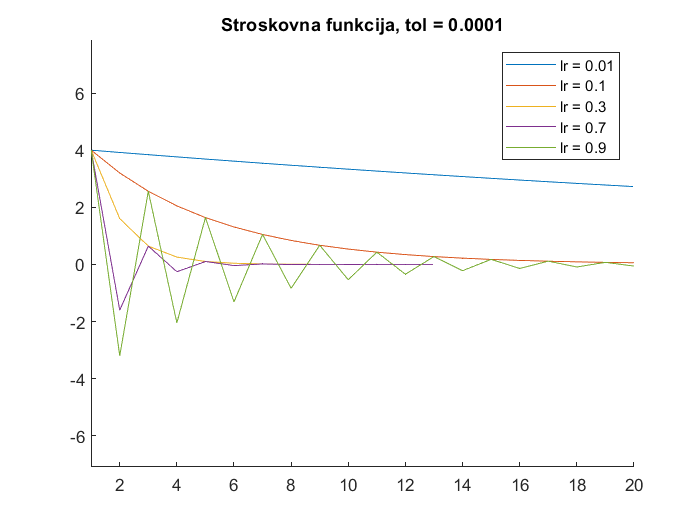
\includegraphics[scale=0.6]{str_fun}   
 \caption{Izravnana funkcija}
\label{fig:foobar}
\end{figure}

\newpage
\subsection{Iskanje minimuma funkcije več spremenljivk}
Podobno kot pri iskanju minimuma funkcije ene spremenljivke si lahko za začetek pogledamo enostaven primer, torej funkcijo $x^2+y^2$. V primeru, ko je učna stopnja enaka 0.8 lahko opazimo, da tako x koordinate kot y koordinate skačejo iz pozitivnih v negativna števila in dosežejo minimum v 19 iteracijah, med tem ko pri učni stopnji 0.1 so vrednosti obeh koordinat pozitivne in lepo padajo k minimumu. V tem primeru pa je potrebnih 31 iteracij.\\

\begin{figure}[h]
    \centering
    \subfigure{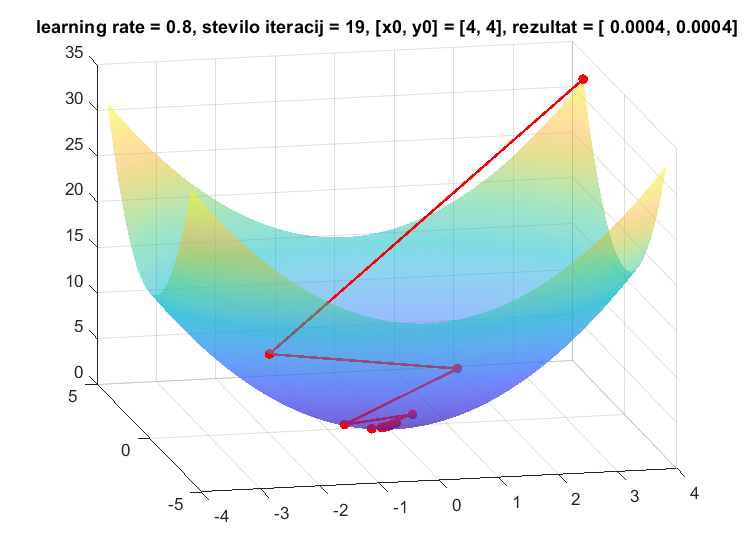
\includegraphics[width=0.45\textwidth]{skacevec.png}}
    \subfigure{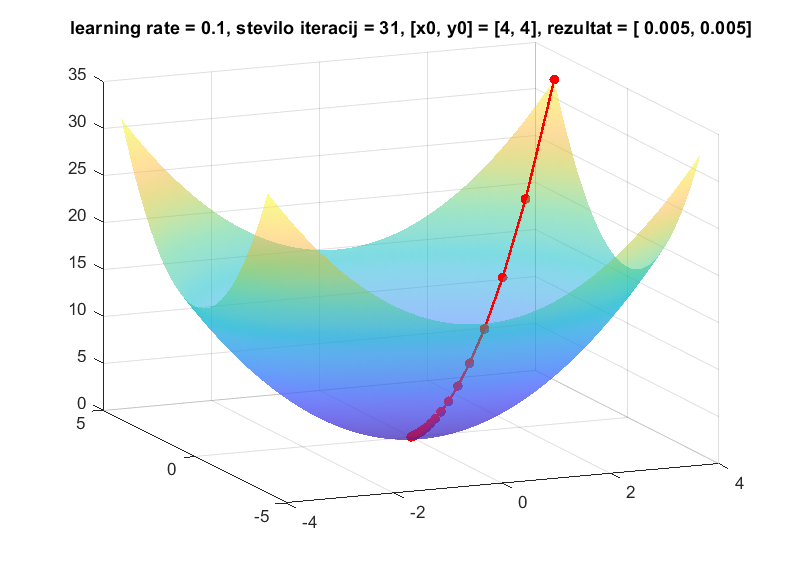
\includegraphics[width=0.45\textwidth]{lepovec.png}} 
    \caption{Razlike glede na izbran learning rate}
    \label{fig:foobar}
\end{figure}


\noindent Če si pogledamo funkcijo, ki ima sedla in več lokalnih ter globalnih minimumov opazimo podobne stvari, kot v primeru funkcij ene spremenljivke. Samo iskanje minimuma je zelo odvisno od izbire začetnega približka in učne stopnje. Na spodnjih grafih opazimo, da pri različnih učnih stopnjah metoda najde različne minimume. Prav tako je razlika v konvergenci, nekje lepo pada proti minimumu, nekje pa skače iz ene strani minimuma na drugo stran.

\begin{figure}[h]
    \centering
    \subfigure{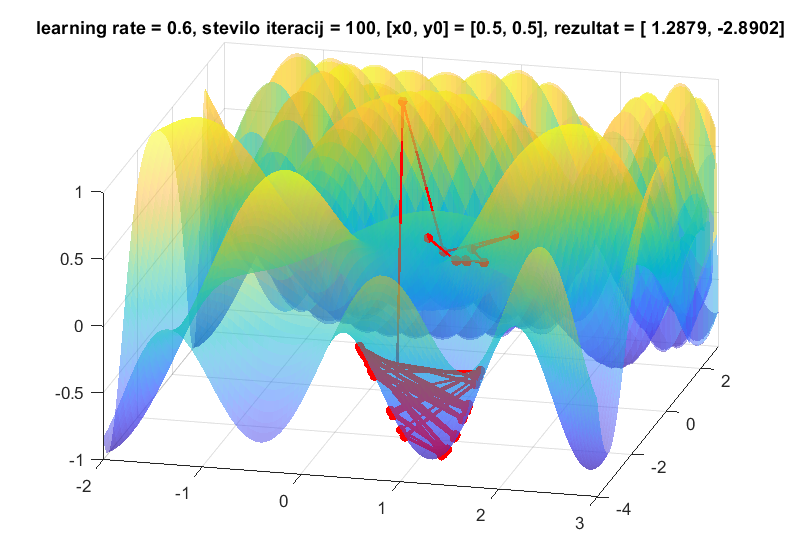
\includegraphics[width=0.45\textwidth]{sedlo1vec.png}}
    \subfigure{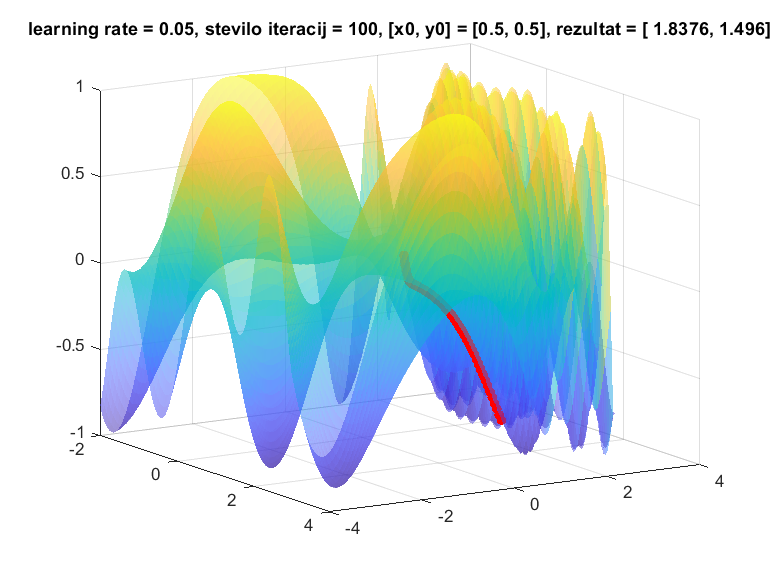
\includegraphics[width=0.45\textwidth]{sedlo2vec.png}} 
    \caption{Razlike glede na izbran learning rate}
    \label{fig:foobar}
\end{figure}

\newpage
\section{Zaključek}
....
%OPOMBE: \\
%
%algoritem je primeren za konveksne funkcije, da ni preveč konstnantna funkcija na nekaterih občmočjih in funkcija ki ne zelo nihajo, kot neke cene delnic. Funkcija mora biti diferenciabilna oz odvedljiva\\
%manjši kot je learning rate dlje traja da skonvergira... \\
%Če je learning rate prevelik lahko algoritem preskoči našo vrednost in ne bo skonvergira \\
%
%Gradientni spus je optimizacijska metoda za iskanje minimuma funkcije s pomočjo iterativnega premikanja v smeri negativnega gradienta.\\


\begin{thebibliography}{9}
\bibitem{texbook}
Nisheeth K. Vishnoi (2020) \emph{Algorithms for Convex Optimization}. Pridobljeno 24. 4. 2022 iz \url{https://convex-optimization.github.io/}.

\bibitem{lamport94}
Robert Kwiatkowski (2021) \emph{Gradient Descent Algorithm — a deep dive}. Pridobljeno 30. 4. 2022 iz \url{https://towardsdatascience.com/gradient-descent-algorithm-a-deep-dive-cf04e8115f21}.

\end{thebibliography}
\end{document}